\question[3]
	\textbf{Logic Gates}

	Implement the logic function: $$Z=\overline{(A+B)\cdot(C\cdot D)}$$
	You can only use the logic gates shown in Fig.~\ref{fig:gates}!

	\begin{figure}[h]
		\centering
		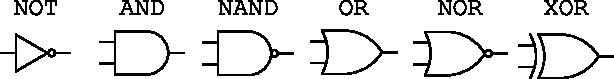
\includegraphics{images/gates.pdf}
		\caption{Available logic gates}
		\label{fig:gates}
	\end{figure}

	\begin{solution}[5cm]
		THIS IS THE SOLUTION
		
		% use this for hiding solution images
		% see: http://www-math.mit.edu/~psh/exam/examdoc.pdf
		% Section 8.3 
		\ifprintanswers
			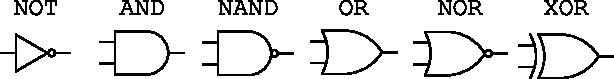
\includegraphics{images/gates.pdf}
			\captionof{figure}{Available logic gates}
			\label{fig:gates}
		\fi
		
	\end{solution}
